\chapter{Evaluation}
kapitelstarttext...
\section{Simulationsaufbau}
Zunächst wird auf den Aufbau des verwendeten Simulators eingegangen, sowie auf die ,in der Simulationen verwendeten, Daten.
\subsection{Simulationsframework und Simulatoren}
Für die Durchführung der Simulation der in Kapitel 3 vorgestellten Methodiken wird die co-Simulations Software Mosaik \footnote{https://mosaik.offis.de/} verwendet. Der Mosiak Simulator wurde speziell für Simulation von Smart Grid-Anwendung entwickelt und eignet sich deswegen hervorragend für die im Zuge dieser Arbeit zu erfüllenden Aufgaben. Der Simulator unterstütz zudem die schchnelle Einbing von einem Framework namens PYPOWER. PYPOWER wurde zur Simulation von Stromflüssen entwickelt und ist in der Lage anhand eines Stromnetzes die Ströme der elektrischen Energie zu simulieren. Diese Simulationdes Stromflusses schließt auch den Transportverlust der Niederspannung und den Zusammenhang von Wirk- zu Blindleistung mit ein. Die Art der Integration von PYPOWER in die Mosaik co-Simulations Software, sorgt dafür, dass ein Nutzer PYPOWER nicht außergewöhnlich konfigurieren muss. Ein Stromnetz welches an Mosaik übergeben wird, wird automatisch PYPOWER mitverwenden. Das Stromnetz welches in dieser Arbeit verwendet wird ist ein standardisiertes europäisches Niederspannungsnetz, welches von der IEEE, dem Institut für Elektro- und Elektronikingenieure, für solche Simulation herausgegeben wurde, um Ergebnisse auf einer EU-weiten Ebene vergleichbarer zu machen. Die Methodiken um den Stromfluss im Niederspannungsnetz zu beeinflussen wurden im Kapitel 3 vorgestellt. Dieser Teil des Simulators ist auch der einzige Teil welcher zwischen den verschiedenen Simulationen ausgetauscht wird. Der letzte Baustein welcher für die Simulation benötigt wird, sind die Fahrzeuge, welche geladen werden sollen. Dieser Simulator ist in der Lage anhand der aus dem Netz abgerufen Leistung und der Zeit zu bestimmen, wie sich die Fahrzeugparameter verändern. Die verschiedenen Teile des Simulators benötigen an manchen Stellen Daten von anderen Teilen des Simulators. Die Methodiken, welche in dieser Arbeit entwickelt wurden setzen an den Anschlusspunkten des Niederspannungsnetzes für Privatverbraucher an. Über diese Anschlusspunkte wird unter anderem die Leistung bezogen, welche für das laden der mit diesem Anschlusspunkt verbunden Elektrofahrzeuge verwendet wird. Die aktuell verwendete Methodik erhält vom jeweiligen Anschlusspunkt die aktuell anliegende Spannung. Die mit dem jeweiligen Anschlusspunkt verbunden Elektrofahrzeuge, teilen der Methodik die Ankunftszeit, den Abfahrtszeitunkt, die aktuell möglich Stromstärke beim Laden, sowie den aktuellen Ladestand mit. Das jeweilige Elektrofahrzeug bezieht dann die von der Methodik berechnete mögliche Ladeleistung aus dem Netz, teilt diesem also die Höhe der bezogenen Leistung mit. Die Transformatorlast wird über ein Broadcastsystem vom Transformator aus verteilt, Die Teilnehmeranzahl kann von jeder Methodik, anhand der erhaltenen Nachrichten bestimmt werden. Diese Nachrichten wurden wiederrum von anderen Teilnehmer versandt.\\
\begin{figure}[htb]
\centering
	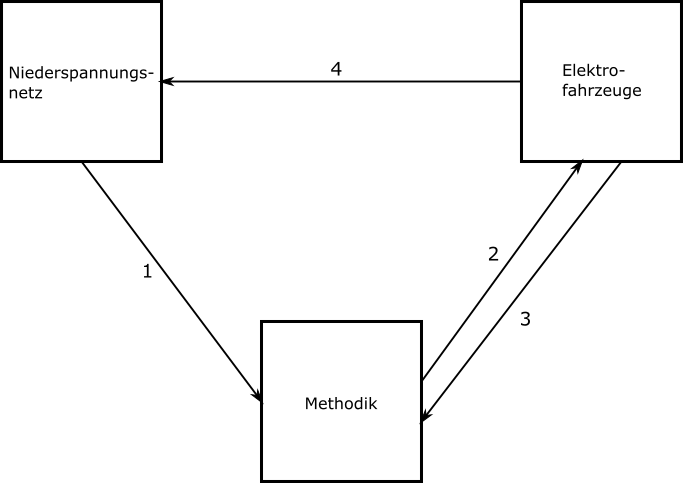
\includegraphics[width=0.5\textwidth]{img/SimAufbau1.png}
	\caption{Schnittstellen zwischen den Teilen des Simulators}
	\label{Abb_SimAufbau}
\end{figure}

In der Abbildung \ref{Abb_SimAufbau} wird ersichtlich wer welche Daten an wen weitergibt. Die mit der eins markierte Verbindung stellt die Weitergabe von Daten  vom Niederspannungsnetz an die aktuelle verwendete Methodik dar. Dabei wird die aktuell am Anschlusspunkt gemessene Spannung weitergegeben. Die zwei mit zwei und drei markierten Übergänge verdeutlichen den Datenaustausch zwischen der verwendeten Methodik und dem angeschlossen Elektrofahrzeug. Das Elektrofahrzeug sendet die Ankunftszeit, die Abfahrtszeit, die aktuell maximal mögliche Stromstärke und den Ladezustand an die Methodik und erhält im Gegenzug die aktuelle Höhe der aus dem Netz beziehbaren Leistung. Über die Verbindung, welche mit 4 markiert ist, wird dem Netz von Elektrofahrzeug mitgeteilt, welche Leistung aktuell aus dem Netz bezogen wird.
\subsection{Annahmen und verwendete Daten}
Im Zuge dieser Arbeit wird eine nicht unerhebliche Menge an Daten verarbeitet. Die Mehrheit dieser Daten steht in Zusammenhang mit den Elektrofahrzeugen. Die Daten die diese für die Simulation zur Verfügung stellen, wurden vom Deutschem Zentrum für Luft – und Raumfahrt erhoben. Diese Erhebung fand im Zuge einer Mobilitätsstudie statt. Es wurden Teilnehmer für diese Studie aus der Bevölkerung ausgewählt, welche dann ihr Mobilitätsverhalten dokumentiert haben. Diese Mobilitätsverhalten dienen als Grundlage für die Daten der verwendeten Elektrofahrzeuge. Durch die Auswertung dieser Daten wurden Ankunfts- und Abfahrtszeiten, sowie die jeweils gefahrene Wegstrecke bestimmt. Durch die Länge der Wegstrecke kann bestimmt werden wie viel des Ladezustandes auf dieser Strecke verbraucht wird und somit auch der Ladestand bei Ankunft an der Ladestation.\\
Es werden für die Simulationen auch einige Annahmen getroffen. Der Kapazität der Batterie, in welcher die elektrische Energie der Elektrofahrzeuge gespeichert wird, wird auf 36253,11 Wh festgelegt. Dieser Wert durch Auswertung zweier Statistiken ermittelt, welche die meistzugelassen Elektrofahrzeuge in Deutschland beinhalteten und die Batteriekapazität pro Modell. Durch die Verwendung dieser Statistiken wurde eine durchschnittliche Batteriekapazität der Elektrofahrzeuge in Deutschland ermittelt. Dieser Mittelwert stellt einen Kompromiss zu einer individuellen Batteriekapazität dar, stellt allerdings auch sicher vergleichbare Ergebnisse zu erhalten. Die Norm DIN EN 50150 setzt die Normspannung im Deutschem Stromnetz auf 230 Volt, daher wird dieser auch in dieser Arbeit verwendet. Die maximale Trafolast wurde durch eine Simulation ohne Aktivität von Elektrofahrzeugen ermittelt. Die, in dieser Simulation gemessene, Transformatorlast wurde verdoppelt. Diese Verdopplung soll die Belastung des Transformators so gering wie möglich halten, den Ladevorgängen aber dennoch die Möglichkeit bieten auch Leistung abzurufen. Eine weitere Annahme ist die maximale Anzahl an Elektrofahrzeugen, hierbei wurde davon ausgegangen, das ein jeder Haushalt im Niederspannungsnetz über exakt zwei Elektrofahrzeuge verfügt, welche mithilfe eine 22kW Ladegeräts geladen werden. Diese Annahme geht aus Statistiken eines Bundesamtes zurück, welche aussagt, das in ländlich geprägten Gebieten vermehrt größere Haushaltemit zwei oder mehr Personen auftreten. Aus Gründer der Normalisierung zwischen den Anschlusspunkten ans Niederspannungsnetz, wird daher immer von zwei Fahrzeugen je Anschlusspunkt ausgegangen. bei dem in dieser Arbeit verwendtem Netz dem IEEE906 gibt es 55 Anschlüsse für Haushalte, folglich wird von 110 Elektrofahrzeugen ausgegangen.

\section{Simulationsergebnisse}
Die Ergebnisse der Simulationen werden zunächst aufgeteilt auf die verwendeten Methodiken vorgestellt. Eingegangen wird auf die verursachte Trafolast, die Spannungen, aufgetretene und behandelte Kollisionen, sowie die Qualitätserfahrungen und die Fairness zwischen den Ladevorgängen. 
\subsection{VDE alleine}
Abbildung \ref{Abb_VDEtauTrafoLast} zeigt die Transformatorlast über den Zeitraum von einer Woche unter Verwendung eines dezentralen VDE Spannungs-Controllers, wie er in Kapitel \ref{capBody:VDE} eingeführt wurde. Ebenso ist die Grundlast, welche unabhängig der Elektrofahrzeuge auftritt.
\begin{figure}[htb]
\centering
	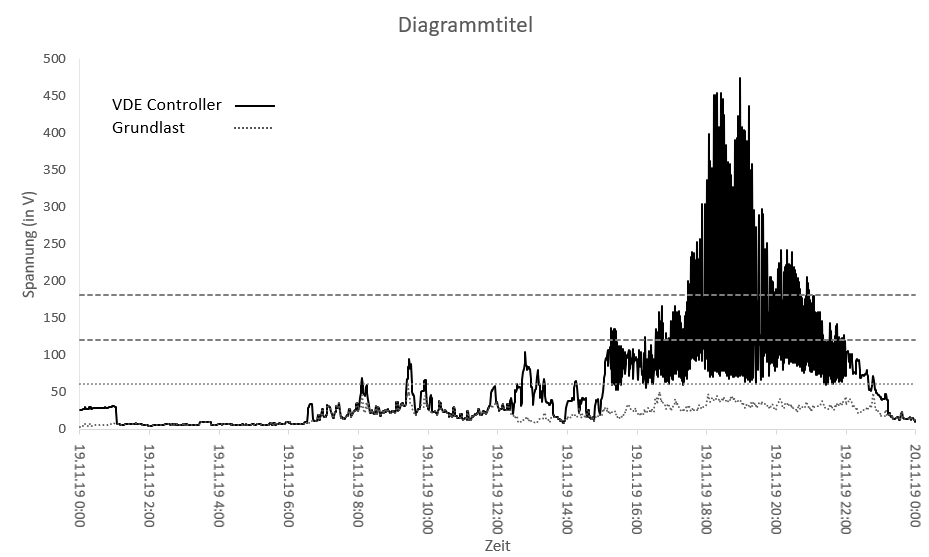
\includegraphics[scale=0.7]{img/VDE_tau/TrafoLast6.png}
	\caption{Trafolast bei Verwendung des VDE Spannungs-Controllers}
	\label{Abb_VDEtauTrafoLast}
\end{figure}

Die gestrichelte, untere vertikale Linie markiert die maximale Last, 60,5 kVA auf der Y-Achse, welche ohne Aktivität der Elektrofahrzeuge am Netz anliegt. Die beiden gepunkteten Linien stellen den Bereich von doppelter bis dreifacher Nominallast dar. Je mehr VA an Scheinleistung der Transformator ans Niederspannungsnetz abgeben muss, desto höheren Lasten ist der Transformator ausgesetzt. Die gepunktete kurve stellt die Höhe der Grundlast dar. Die Grundlast deckt jeglichen Verbrauch von elektrischer Energie außerhalb des Ladens von Elektrofahrzeugen ab. Der VDE Controller gibt an, wie viel Energie insgesamt durch das Laden von Elektrofahrzeugen und die Grundlast verbraucht wird. \\
Die Abbildung stellt die Werte des dritten von sieben Tagen der Simulation dar. Die bereits erhöhte Last zu Beginn des Zeitraums lässt darauf schließen, dass Fahrzeuge welche bereits am Tag zuvor angekommen sind noch immer laden. Im Zeitraum von 8:00 bis 10:00 steigt sowohl die Grundlast aber auch die Last an sich an, Die Nähe der beiden Kurven lässt allerdings auf eine geringe Anzahl von Ladevorgängen schließen. Von etwa 12:00 bis 14:00 und 14:00 bis 14:30 sind an der Leistungskurve aufgrund der Erhöhung zur Grundlast erstmals Ladevorgänge deutlich erkennbar. Von 15:00 bis 23:00 ist durchweg ein hoher Mehrverbrauch von Energie sichtbar. Die Leistungskurve liegt hier deutlich über der Grundlast, bei einer stabilen Grundlast von etwa 30 bis 40 kVA wird der Verbrauch durch das Laden auf teilweise etwa 450 kVA mehr als verzehnfacht. In dem Zeitabschnitt liegen die Messungen fast ausschließlich über der maximal gemessen Grundlast. Am Aussehen des Graphen in diesem Zeitraum, lässt sich eine starke Oszillation der erhaltenen Werte erkennen. Da ein solches Verhalten nur in Situationen mit einer hohen Last auftritt, bedeutet das der verwendete Controller mit eben solchen Situationen nicht umgehen kann. Da solch hohe Lasten durch das Laden von Elektrofahrzeugen jedoch häufiger vorkommen und der Controller nicht in der Lage ist das Leistungsniveau dauerhaft zu senken, stellt dies seine Verwendbarkeit an sich in Frage. \\
Über dem gesamten  Zeitraum der Simulation wurde die Grenze von 121 kVA in 7,3 \% der betrachteten Zeit überschritten. Die Überschreitungen traten verteilt auf. Die vorherige maximale Last von 60,5 kVA wurde dabei sogar 25,2 \% der Zeit überschritten. Die maximal gemessene Last beträgt etwa 475 kVA. Solche Spitzenwerte können kaum vermieden werden, wenn mehrere Fahrzeuge gleichzeitig zu Laden beginnen. Da ein einzelnes Fahrzeug nur dezentral entscheiden kann. Die im Mittel abgegeben Last beträgt etwa 45,1 kVA. Wenn nur die Grundlast betrachtet wird, beträgt die mittlere abgegeben Leistung etwa 20,5 KVA, somit nimmt sie etwa 45 \% der mittleren Trafolast in Anspruch. Am Graphen ist erkennbar, dass ein Anstieg der Grundlast meist auch einen Anstieg der eigentlichen Last nach sich zieht. Daraus lässt sich folgern, dass bei Zeitpunkten mit hoher Grundlast auch vermehrt Elektrofahrzeuge zu laden beginnen bzw. ladebereit sind. Die Passagiere der angekommenen Elektrofahrzeuge, benötigen neben der Energie zum Laden der Elektrofahrzeuge auch Energie für den persönlichen Gebrauch, somit steigen die Grundlast zusätzlich zur neu hinzugekommen Last durch das Laden an. 

\begin{figure}[htb]
\centering
	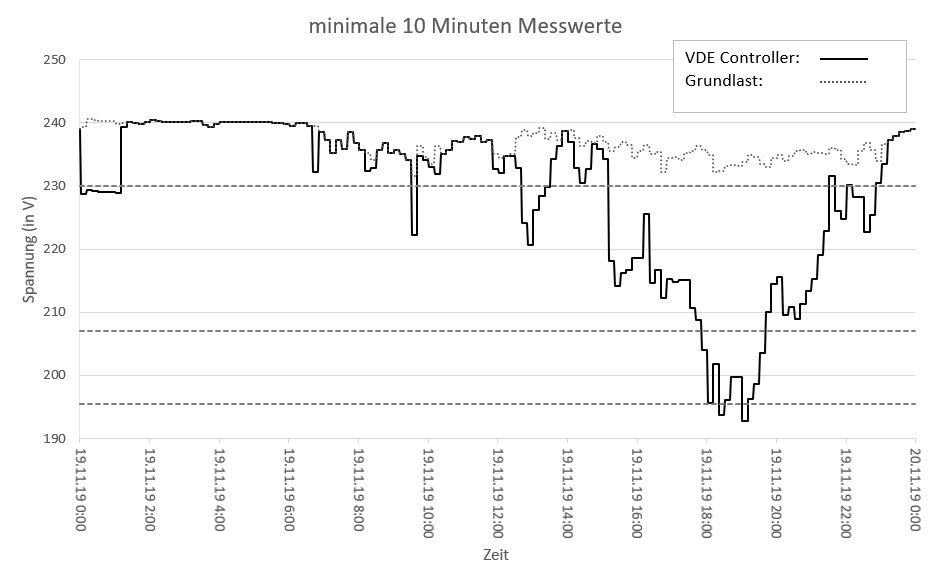
\includegraphics[scale=0.7]{img/VDE_tau/Spannung10m5.png}
	\caption{Spannungsverlauf mit 10 Minuten Mittelwerten bei Verwendung des VDE Spannungs-Controllers}
	\label{Abb_VDEtauSpannung10m}
\end{figure}

In Abbildung \ref{Abb_VDEtauSpannung10m} ist der selbe Experiment dargestellt wie in Abbildung \ref{Abb_VDEtauTrafoLast}. Dargestellt sind ist der jeweilige Minimalwert der Spannung über alle Anschlusspunkte. Die einzelnen Messwerte werden für jeden Anschlusspunkt individuell erfasst. Die Spannung wird aber nicht in jeder Minute aktualisiert, sondern Daten werden in 10 Minuten Intervallen gesammelt und deren Mittelwert wird abgebildet. 10 Minuten Mittelwerte, wurden gewählt, um die Spannungsqualität gemäß DIN EN 50160 zu bewerten. Die Norm gibt vor das über einen Zeitraum von einer Woche zu mindesten 95 \% der Zeit ein Spannungswert von mehr als 95 \% der Normspannung von 230V, gemessen werden muss. Der Grenzwert von 95 \% der Normspannung ist durch die mittlere gestrichelte Linie markiert. Die verblieben 5 \% der Zeit darf die Spannung sogar um bis zu 15 \% absinken. Dieser Grenzwert darf allerdings nicht weiter unterschritten werden. Die untere gepunktete Linie markiert 85 \% der Normspannung. Zur Einordnung zeigt die oberste, vertikale gestrichelte Linie die Normspannung von 230 V an. Der gepunktete Graph zeigt den verlauf der minimalen Spannung, wenn nur die Grundlast bezogen wird. Die durchgezogene Line zeigt den minimalen Spannungsverlauf wenn neben dem bezug der Grundlast auch Elektrofahrzeuge geladen werden.\\
Das Absinken der Spannung korreliert mit dem Anstieg der bezogen Leistung. In dem Zeitraum in dem vermehrt Leistung bezogen wird, siehe Abbildung \ref{Abb_VDEtauTrafoLast}, sinkt auch die Spannung ab. Da in dieser Spannung die Minimalwerte über das gesamte Niederspannungsnetz hinweg betrachtet werden, tritt hier keine Oszillation auf. Im Zeitraum von etwa 18:00 bis 20:00 ist eine Unterschreitung der 207 V Markierung erkennbar, somit liegt der Minimal Wert in etwa 7\% der Zeit unter 207 V Grenze. Diese Unterschreitung ist allerding nicht aussagekräftig, da die Norm DIN EN 50160 einen Zeitraum von einer Woche und nicht von einem Tag betrachtet. In demselben Zeitraum ist allerdings auch eine Unterschreitung der 195,5 V Markierung erkennbar. Eine solche Unterschreitung ist in der Norm generell nicht vorgesehen, somit ist Norm nicht erfüllt.\\
Der niedrigste gemessene Mittelwert im gesamten betrachteten Netz liegt bei 192,86 V, dies entspricht einer Unterschreitung von 230 V um 16,8 \%. Dies verstößt gegen den zweiten Teil der Norm. Der erste Teil wird aber erfüllt, die maximale Anzahl an Unterschreitungen der 107 V Grenze beträgt 21, was etwa 2,1\% der Zeiten entspricht. Der mittlere gemessene Wert liegt bei 234,06 V, dies liegt sogar über der Normspannung. Dies lässt darauf schließen, dass die Einspeisespannung des Transformators mehr als 230 V beträgt.
Neben den 10 Minuten Mittelwerten, werden auch die Minutengenauen Werte der Spannung erfasst. Der niedrigste einzelne Messwert der Spannung liegt bei 152,23 V.  Dieser Wert liegt nochmal deutlich unter dem Minimum der 10 Minuten Mittelwerte. Der mittlere Spannungswert über das gesamte Niederspannungsnetz liegt bei 234,06 V lediglich 3,5\% (8,36 \%??) Standardabweichung. Die mittleren Werte der einzelnen Spannungsmessungen und der 10 Minuten Werte stimmen also überein. \\

Die hier vorgestellte Methodik reagiert auf keine Art von Kollision, dennoch wurde die Anzahl von Situationen erfasst, in denen Kollisionen aufgetreten wären. Hierbei gibt es zu beachten, dass der Simulationszeitraum 10080 Schritte umfasst, welche von jedem der 110 betrachteten Fahrzeuge durchlaufen werden. Dies bedeutet es werden 1108800 Situationen betrachtet. In 0,13 \% davon ist eine Spannungskollision aufgetreten und in 0,15 \% davon ist eine Transformatorkollision aufgetreten. In insgesamt 0,15 \% der Fälle, also 5615 Situationen, trat eine Art von Kollisionen auf. Diese Arten der Kollisionen beinhalten eine reine Spannungskollision, eine reine Transformatorkollision, sowie eine Spannungskollision und Transformatorkollision, welche zeitgleich auftreten. \\
Innerhalb des Simulation Zeitraumes werden insgesamt 557 Ladeservices gestartet, von denen alle erfolgreich abgeschlossen wurden. Dies bedeutet, dass ein jedes Fahrzeug beim Verlassen der Ladestation einen Ladezustand von 100 \% aufwies. Beim Start eines Ladeservices lag der durchschnittliche Ladestand bei etwa 85 \%, schon nach etwa 40 \% des Ladeservices liegt der durchschnittliche Ladestand bei fast 100 \% mit einer Standardabweichung von lediglich 0,8 \%. 
\begin{figure}[htb]
	\centering
	\begin{minipage}[t]{0.49\linewidth}
		\centering
        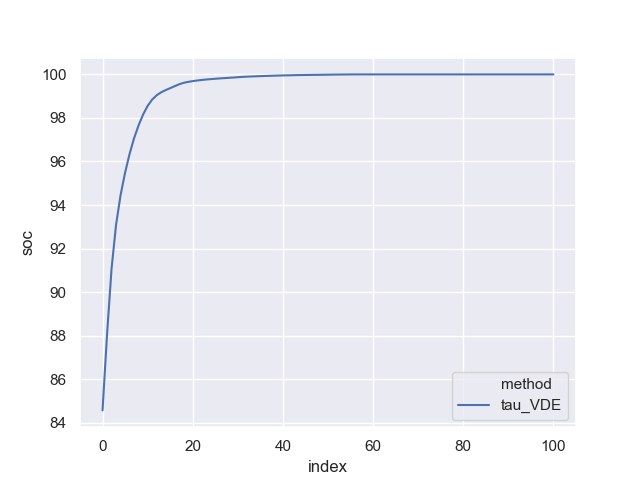
\includegraphics[width=\linewidth]{img/VDE_tau/tau_VDE_2_soc_mean.png}
        \caption{Durchschnittlicher Ladezustand eines Elektrofahrzeuges}
        \label{ABB_VDEtauSocMEAN}
	\end{minipage}
	\hfill
	\begin{minipage}[t]{0.49\linewidth}
		\centering
        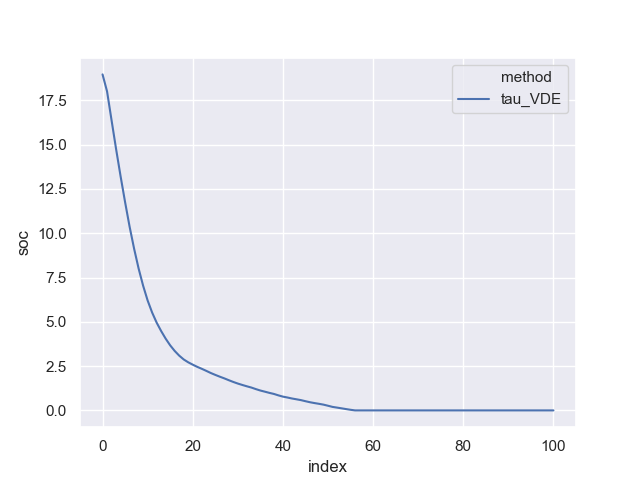
\includegraphics[width=\linewidth]{img/VDE_tau/tau_VDE_2_soc_std.png}
        \caption{Durschschnittliche Standardabweichung des Ladezustandes}
        \label{ABB_VDEtauSocSTD}
	\end{minipage}
\end{figure}

Da alle begonnen Ladeservices erfolgreich beendet wurden, ist die Qualität der Ladeservices maximal. Die Fairness beim Erreichen dieser Qualität ist in Abbildung \ref{Abb_VDEtauFairness} aufgezeichnet. \\
\begin{figure}[htb]
\centering
	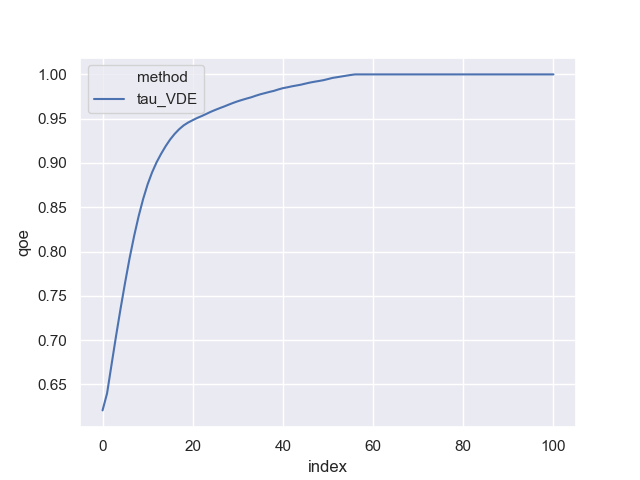
\includegraphics[scale=0.4]{img/VDE_tau/tau_VDE_2_qoe.png}
	\caption{Durchschnittlicher Qualitätserfahrung eines Elektrofahrzeuges}
	\label{Abb_VDEtauFairness}
\end{figure}

Die Fairness wird mithilfe der Hoßfeld Methode \cite{Hosfeld2018} berechnet. Diese Methode bezieht die Standardabweichung vom Ergebnis als auch die maximal und minimal möglichen Werte des Ergebnisses mit ein. Der Wert der Fairness wird mit folgender Formel F($\sigma$) berechnet.
\begin{align}
	F(\sigma) = 1-\frac{2*\sigma}{100}
\end{align}

$\sigma$ steht für die Standardabweichung des Ladezustandes beim Verlassen der Ladestation. Die 100 im Nenner des Bruches kommt zustande durch die Subtraktion des niedrigsten möglichen Wertes vom höchst möglichen Wert, 100 – 0. Das Ergebnis der Formel liegt im Bereich von 1 bis 0, (0,1). Je höher das Ergebnis der Formel, desto höher ist die Fairness zwischen den Teilnehmern. Die zu Beginn niedrigere Fairness lässt sich auf die zu Beginn auch hohe Standardabweichung beim Ladestand der einzelnen Fahrzeuge zurückführen. Je geringer die Standardabweichung allerdings wird, desto höher steigt auch der Wert der Fairness.

\subsection{SA-Part alleine}
Fülltext über Fülltext, nur damit ich sehe wie es mir die Bilder bei mehr Text noch verschieben würde. Fülltext über Fülltext, nur damit ich sehe wie es mir die Bilder bei mehr Text noch verschieben würde. Fülltext über Fülltext, nur damit ich sehe wie es mir die Bilder bei mehr Text noch verschieben würde. Fülltext über Fülltext, nur damit ich sehe wie es mir die Bilder bei mehr Text noch verschieben würde. Fülltext über Fülltext, nur damit ich sehe wie es mir die Bilder bei mehr Text noch verschieben würde. Fülltext über Fülltext, nur damit ich sehe wie es mir die Bilder bei mehr Text noch verschieben würde. Fülltext über Fülltext, nur damit ich sehe wie es mir die Bilder bei mehr Text noch verschieben würde. Fülltext über Fülltext, nur damit ich sehe wie es mir die Bilder bei mehr Text noch verschieben würde. Fülltext über Fülltext, nur damit ich sehe wie es mir die Bilder bei mehr Text noch verschieben würde. Fülltext über Fülltext, nur damit ich sehe wie es mir die Bilder bei mehr Text noch verschieben würde.
\subsection{SA-waitingTime alleine}
\subsection{SA-Part-trafo alleine}
\subsection{SA-waitingTime-trafo alleine}
\section{Analyse und Auswertung}
\subsection{SA-part mit SA-waitingTime}
\subsection{SA-part-trafo mit SA-waitingTime-trafo}
\subsection{VDE mit (SA-part, SA-waitingTime)}
\subsection{(SA-part, SA-waitingTime) mit (SA-part-trafo, SA-waitingTime-trafo)}
